\section{Vorlesung 01.06.2016}

\subsection{Struktur -- Funktion: Molekulare Ausstattung von Neuronen}
\begin{itemize}
	\item molekulare Grundausstattung verschiedener Neuronentypen ist weitgehend ähnlich, auch artübergreifend
	\item Grundlage ist intra- extrazellulärer Ionengradient
	\item Membranpotentiale werden durch selektive Permeabilitätsänderungen kontrolliert
\end{itemize}

\subsection{ATPasen}
 - Diese Ionenpumpen bereiten den Boden für die Neuronenfunktion
\\\\
\textbf{Na/K-ATPase}\footnote{\url{https://de.wikipedia.org/wiki/Natrium-Kalium-Pumpe}}
\begin{itemize}
	\item drei Na$^+$-Ionen nach außen und zwei K$^+$-Ionen nach innen befördert
\end{itemize}

\textbf{Mg$^2+$-abhängige Ca-ATPase}
\begin{itemize}
	\item Ca-Transport aus der Zelle
\end{itemize}

\subsection{Ionenkanäle}
\textbf{ - }können je nach Konformation die Permeabilität der Membran selektiv für spez. Ionen ändern. Diese Modulierbarkeit der Kanaleigenschaften ist das eigentliche Wesen der Informationsverarbeitung durch die Zelle\\
\textbf{ - }Innerhalb von msec wechselt der einzelne Kanal zufällig zwischen offenem und geschlossenem Zustand. Was sich spezifisch als Reaktion des Kanals ändert ist die mittlere Öffnungszeit des Kanals\\

\subsubsection{spannungsabhängige Ionenkanäle}
\begin{itemize}
	\item Änderung des Membranpotentials
	\item $\alpha$- und $\beta$- UE ($\alpha$: Pore, $\beta$: modulatorisch)
	\item S4: wichtig für Öffnungsvorgang, Mutagenese ändert Spannungsabhängigkeit des Kanals
	\item S5/6: der Pore am nächsten, bestimmen Selektivität und Leitfähigkeit im geöffneten Zustand
\end{itemize}

\subsubsection{Ligandenabhängige Ionenkanäle (Transmitterrezeptoren)}
 - Bindung eines spezifischen Liganden\\
\\
\textbf{Nikotinischer Acetycholin-Rezeptor}
\begin{itemize}
	\item Tetra- /Pentamer (2$^\alpha$ :$\beta$:$\gamma$:$\delta$) (Neuron: nur $\alpha \beta$; $\delta$-Muskelspezifisch)
	\item $\alpha$ bindet Transmitter , je UE 4 Transmembranbereiche)
	\item jede UE wird von einem Gen kodiert (hochgradig homolog)
	\item alternatives Spleißen und differentielle Expression ermöglicht neuronspezifische Antwortcharakteristik
\end{itemize}

\textbf{Inhibitorische Rezeptoren}
\begin{itemize}
	\item Glycin- / Gaba A -Rezeptoren
	\item Pentamer (Gaba-R= 2$\alpha$:2$\beta$: ($\gamma$))
	\item $\beta$ bindet Transmitter, intrazelluläre Phosphorylierung durch cAMP- abhängige Proteinkinase möglich, extrazellulär mit Glycolosierungsstellen
	\item $\alpha$ Bindungstellen für pharmazeutische Drogen
\end{itemize}

\textbf{Ionotrope Glutamatrezeptoren}
\begin{itemize}
	\item ionotrop: Rezeptor = Kanal
	\item Im Vertebraten-ZNS ist Glutamat der wichtigste erregende Neurotransmitter
	\item Tetramere mit 3 TM
\end{itemize}

Unterfamilien:
\begin{itemize}
	\item Nicht-NMDA-Rezeptoren: Vermittelt schnelle Komponente des postsynaptischen Stroms, Leitfähigkeit von wenigen Millisekunden
		\begin{itemize}
			\item AMPA-Rezeptoren
			\item Kainat-Rezeptoren
		\end{itemize}
	\item NMDA-Rezeptoren: Vermittelt langsame Komponente des postsynaptischen Strome, Dauer: einige wenige Millisekunden
\end{itemize}

\textbf{Vielfalt Ionotrope Glutamatrezeptoren}
\begin{itemize}
	\item Heteromultimere
	\item Alternatives Spleißen
	\item RNA-Editing: punktuelle Modifikation der prä-mRNA bezüglich der genomischen Sequenz führt zu Codonwechsel
\end{itemize}

\subsection{G-Protein-gekoppelte Rezeptoren}\footnote{\url{https://de.wikipedia.org/wiki/G-Protein-gekoppelter_Rezeptor}}
 \textbf{- second messenger Prinzip}\\
 - z.B. Transmitterrezeptoren (metabotrope Glutamatrezeptoren, muscarinischer Acetylcholinrezeptor)\\\\
Übertragung des Signals auf:
\begin{itemize}
	\item Ionenkanäle
	\item Adenylatcyclasen
	\item Phospholipase C (u.a.)
\end{itemize}
kann zu lang anhaltenden zellulären Reaktionen/Veränderungen führen\\

3 UE der G-Proteine (GTP-bindende Proteine):
\begin{itemize}
	\item $\alpha$: 40-50 kD , legt Spezifität des G-Proteins fest
		\begin{itemize}
			\item G$_s$ ,G$_i$ ,G$_{olf}$ – Adenylatzyclase
			\item G$_p$ – Phospholipase C, G$_t$ – cGMP-Phosphodiesterase
			\item G$_0$ - Ionenkanal
		\end{itemize}
	\item $\beta$: 35 kD
	\item $\gamma$: 8 kD
\end{itemize}

Beispiel:\textbf{cAMP-System:}
\begin{itemize}
	\item externes Signal (first messenger): Noradrenalin (auf extrazellurären Seite)
	\item Rezeptor: $\beta$-adrenerger Rezeptor
	\item Transduktor: G$_s$
	\item primärer Effektor: Adenylatcyclase
	\item second messenger: cAMP
	\item sekundärer Effekt: cAMP-abhängige Proteinkinase
\end{itemize}
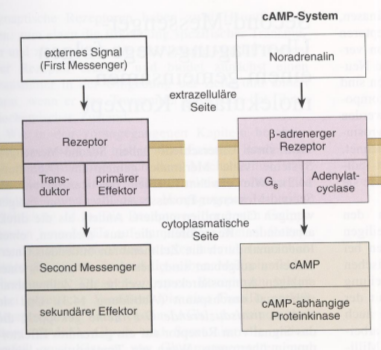
\includegraphics[width=0.6\textwidth]{lectures/160601/pix/1.png}

\subsection{Synaptische Vesikelproteine}\footnote{\url{https://de.wikipedia.org/wiki/Synaptisches_Vesikel}}
Kreislauf in 9 Schritten:
\begin{enumerate}
	\item Docking an Membran
	\item Priming: Vorbereitung für Exozytose (Verbrauch von ATP)
	\item Fusion/Exozytose: bei Aufnahme von Ca$^{2+}$ über kalziumabhängigen Ionenkanal wird die Exozytose eingeleitet und die Neurotransmitter werden in den synaptischen Spalt abgegeben
	\item Endozytose
	\item Translocation: H$^+$-Ionen werden in Visikel aufgenommen und "reservieren" Platz für neue Neurotransmitter
	\item endosome Fusion: Visikel geht in Reservepool über
	\item Budding: Abspaltung eines neuen Visikels
	\item NT uptake: Aufnahe von Neurotransmittern
	\item Translokation: Bewegung innerhalb der Synapse (Plasma) in Richtung Membran
\end{enumerate}